
\documentclass[a4paper,12pt]{article} 
\usepackage[top = 2.5cm, bottom = 2.5cm, left = 2.5cm, right = 2.5cm]{geometry} 
\usepackage[T1]{fontenc}
\usepackage[utf8]{inputenc}
\usepackage{multirow} 
\usepackage{amsmath}
\usepackage{amssymb}
\usepackage{booktabs} 
\usepackage{graphicx}  
\usepackage{subfig}
\usepackage{setspace}
\setlength{\parindent}{0in}
\usepackage{float}
\usepackage{tablefootnote}
\usepackage{fancyhdr}
\usepackage[english]{babel}
\usepackage{xcolor}
\usepackage{multirow}
\usepackage{listings}
\usepackage{dcolumn}
\lstset{
  basicstyle=\footnotesize\ttfamily,
  columns=fullflexible,
  frame=single,
  breaklines=true,
  postbreak=\mbox{\textcolor{red}{$\hookrightarrow$}\space},
}
\usepackage{hyperref}
 \hypersetup{
     colorlinks=true,
     linkcolor=black,
     filecolor=black,
     citecolor = black,      
     urlcolor=blue,
     }
\usepackage{csvsimple}
\pagestyle{fancy} 
\fancyhf{} 
\lhead{\footnotesize Economics 714: PS1}
\rhead{\footnotesize Javier Tasso} 
\cfoot{\footnotesize \thepage} 




\begin{document}





\begin{tabular}{p{15.5cm}} 
{\large \bf Economics 714 - Computational Methods in Economics} \\
University of Pennsylvania \\ Fall 2021 \\ \\ 
\hline 
\\
\end{tabular} 

\vspace*{0.3cm} 

\begin{center} 
	{\Large \bf Problem Set 1} 
	\vspace{2mm}
	
        
	{\bf Javier Tasso} 
		
\end{center}  

\vspace{0.4cm}

%%%%%%%%%%%%%%%%%%%%%%%%%%%%%%%%%%%%%%%%%%%%%%%%
%%%%%%%%%%%%%%%%%%%%%%%%%%%%%%%%%%%%%%%%%%%%%%%%



    % Exercise 1    
    
     
    \section*{Question 1} 
    \medskip

    See \href{https://github.com/javiertasso/econ714_hw1_tasso}{this link}. 

     
    
    % Exercise 2   
    
    \medskip
    \medskip
    \section*{Question 2}     
    \medskip
    
    Figure (\ref{area_part2}) plots the area we want to calculate and table (\ref{table_ex2}) shows the results using different methods. The code \textit{econ714\_homework1\_question2.m} produces these outputs.  
    
    \begin{figure}[!htbp]
        \centering
       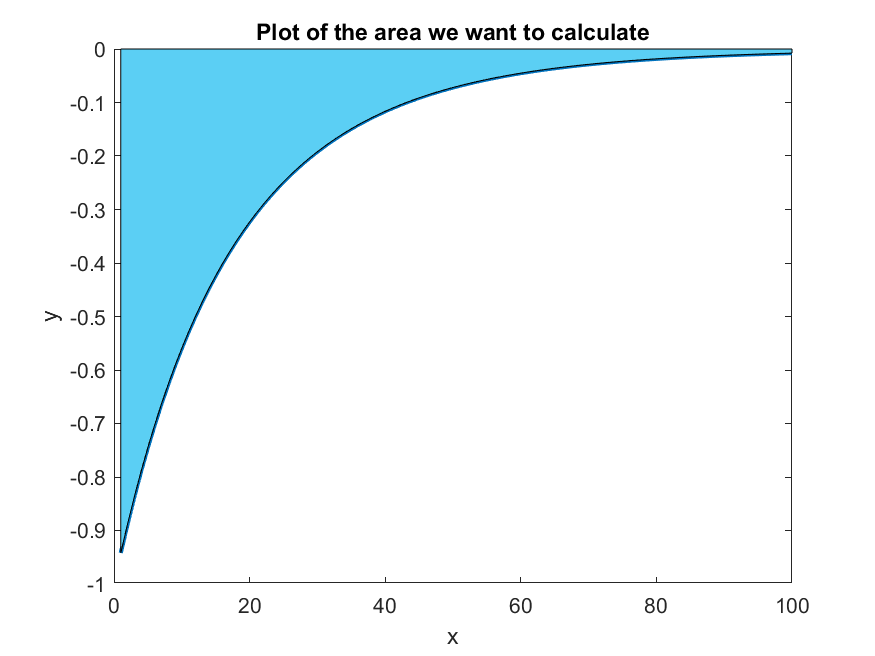
\includegraphics{econ714_homework1_question2_plot.png}
        \caption{Area - Question $2$} 
        \label{area_part2}
    \end{figure}
    
    \begin{table}[!htbp]
        \centering
        \caption[Short Caption for LoT]{Comparison of Different Methods - Integration}\label{table_ex2}
    \csvautotabular{econ714_homework1_question2_output.csv}
    \end{table}
    
 
    
    % Exercise 3   
    
    \medskip
    \medskip
    \section*{Question 3}   
    \medskip
    
    The code \textit{econ714\_homework1\_question3.m} generates the output of question $3$. The function attains a minimum at the point $(1,1)$ and its value is $f(1,1)=0$. We use four initial guesses $(2,3)$, $(2,-3)$, $(-2,3)$ and $(-2,-3)$. 
    
    \begin{itemize}
        \item Newton-Raphson. This algorithm converges in a small number of iterations, but it requires the computation of the inverse of the Hessian, which can be slow as we increase the number of dimensions of the problem. Table (\ref{table_ex3}) shows the number of iterations and time elapsed. 
        
        
        \item BGFS. This algorithm requires more iterations and more times because we are approximating the inverse of the Hessian (without calculating it directly). Table (\ref{table_ex3}) shows the results. We used the following initial guess for the inverse of the Hessian. 
        
        \begin{align*}
            H^{-1}_0 = \begin{pmatrix} \frac{1}{f_{xx}^{''}(1,1)} & 0 \\ 0 & \frac{1}{f_{yy}^{''}(1,1)}  \end{pmatrix} = \begin{pmatrix} \frac{1}{802} & 0 \\ 0 & \frac{1}{200}  \end{pmatrix} 
        \end{align*}
        
        
        
    \begin{table}[!htbp]
        \centering
        \caption[Short Caption for LoT]{Comparison of Different Methods - Minimization}\label{table_ex3}
        \csvautotabular{econ714_homework1_question3_output.csv}
    \end{table}
        
        \item Steepest descent. Figure (\ref{steepest_des_fig}) plots the trajectories for different initial guesses and has the number of iterations and time elapsed included. The algorithm is pretty fast, but since the function is very flat near the minimum the trajectories are not optimal. Circles are the initial guesses and the star is the solution.   
        
        
    \begin{figure}[!htbp]
        \centering
       \subfloat{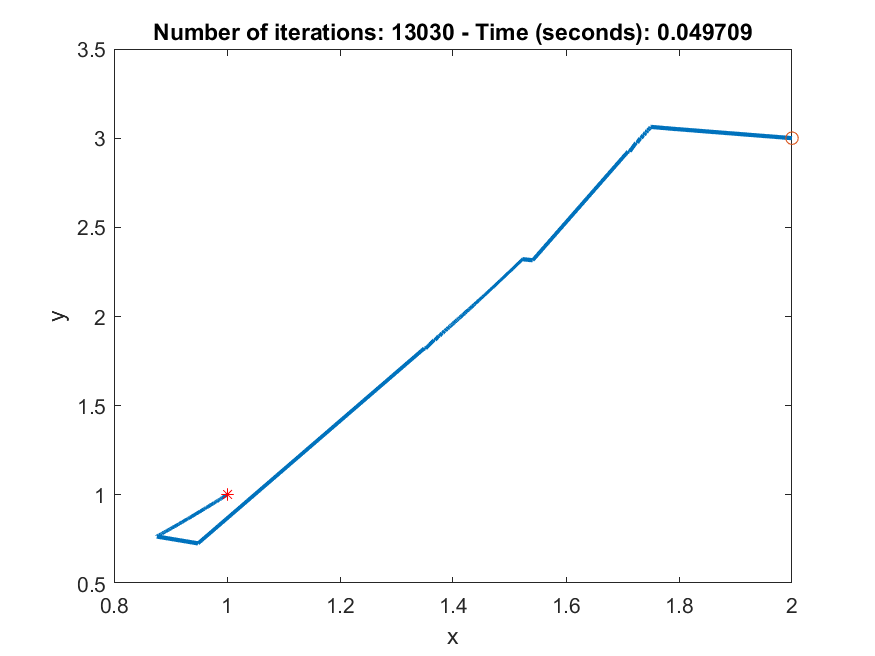
\includegraphics[scale=0.5]{econ714_homework1_question3_plot_steepest_descent_1.png}}
       \subfloat{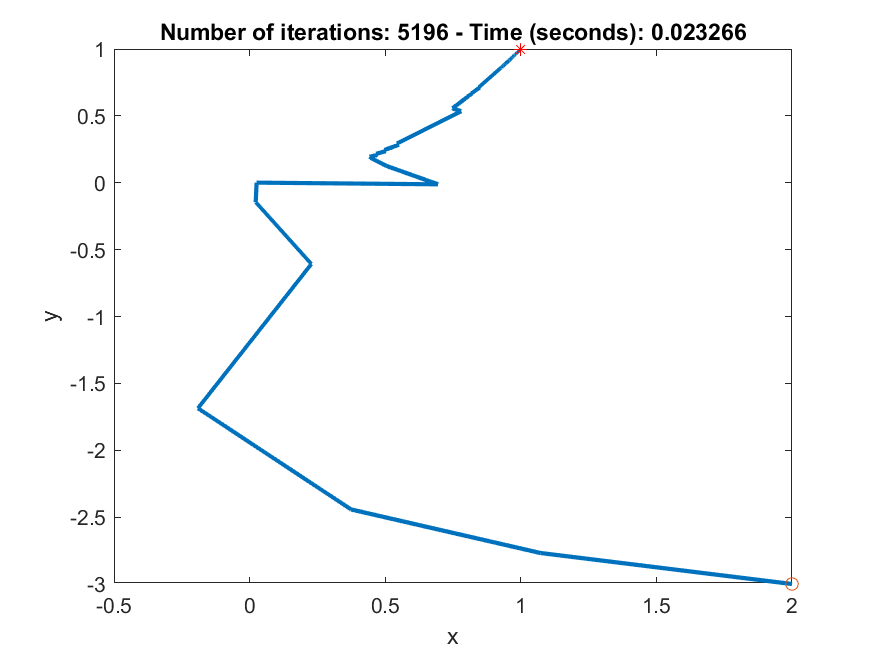
\includegraphics[scale=0.5]{econ714_homework1_question3_plot_steepest_descent_2.png}}
       
       \subfloat{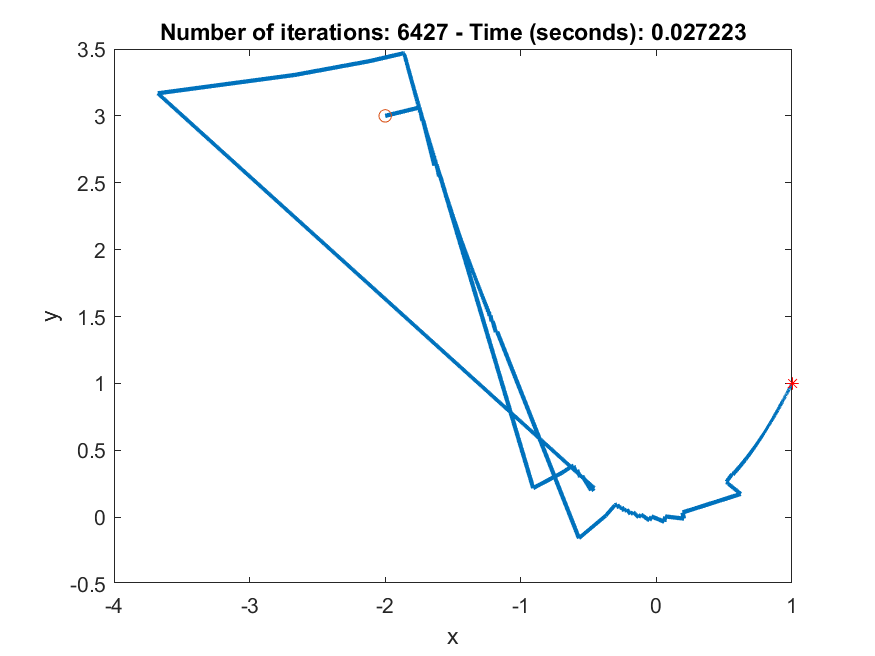
\includegraphics[scale=0.5]{econ714_homework1_question3_plot_steepest_descent_3.png}}
       \subfloat{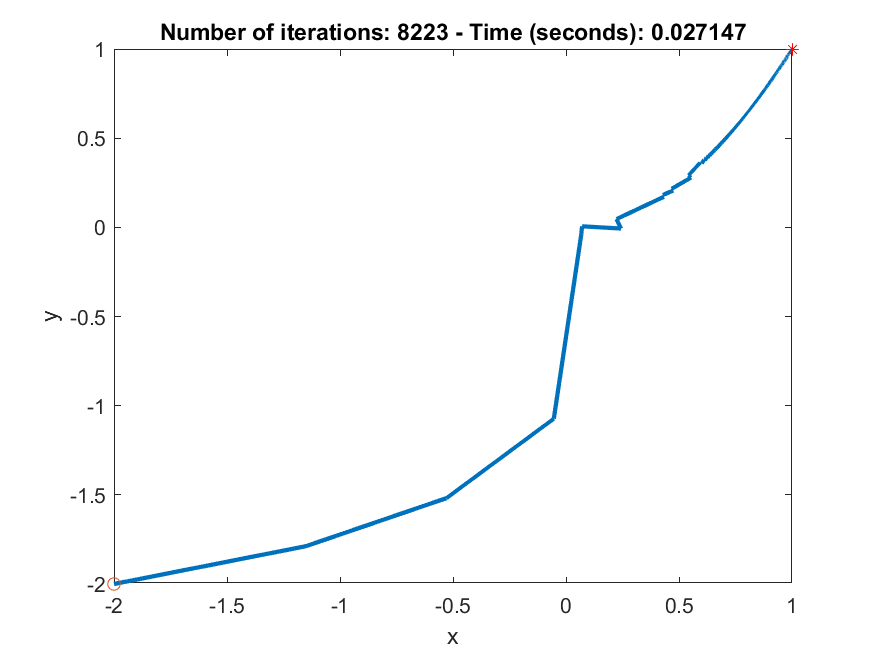
\includegraphics[scale=0.5]{econ714_homework1_question3_plot_steepest_descent_4.png}}
        \caption{Steepest Descent Method} 
        \label{steepest_des_fig}
    \end{figure}
        
        
        
        \item Conjugate descent. Figure (\ref{conj_descent}) shows the results. This one is slower but we see that the trajectories seem smoother. We implemented the non-linear version and as step size we used the inverse of the maximum eigenvalue of the Hessian matrix at the initial guess. As before, circles are the initial guesses and the star is the solution.   
        
        
       \begin{figure}[!htbp]
        \centering
       \subfloat{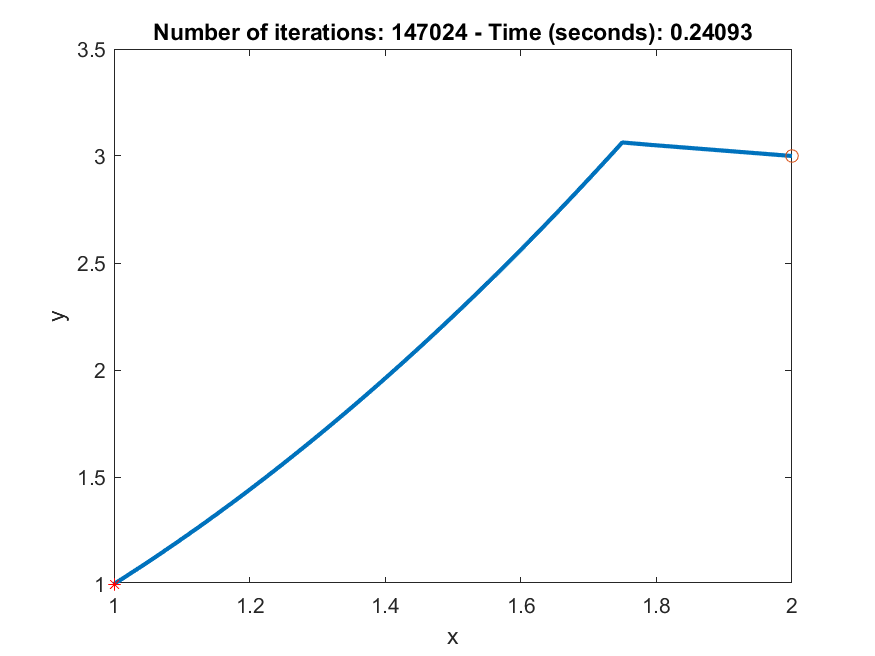
\includegraphics[scale=0.5]{econ714_homework1_question3_plot_cong_1.png}}
       \subfloat{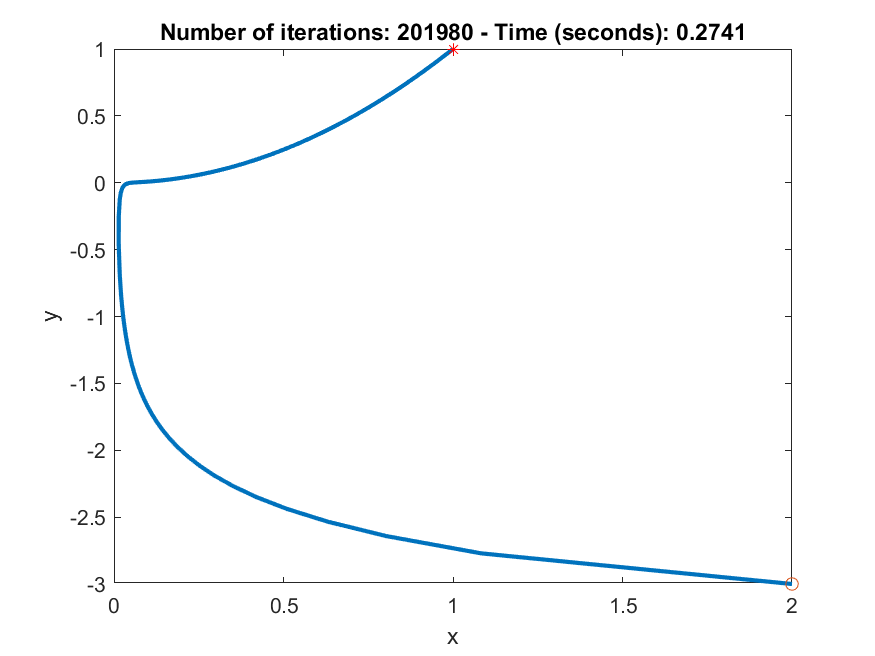
\includegraphics[scale=0.5]{econ714_homework1_question3_plot_cong_2.png}}
       
       \subfloat{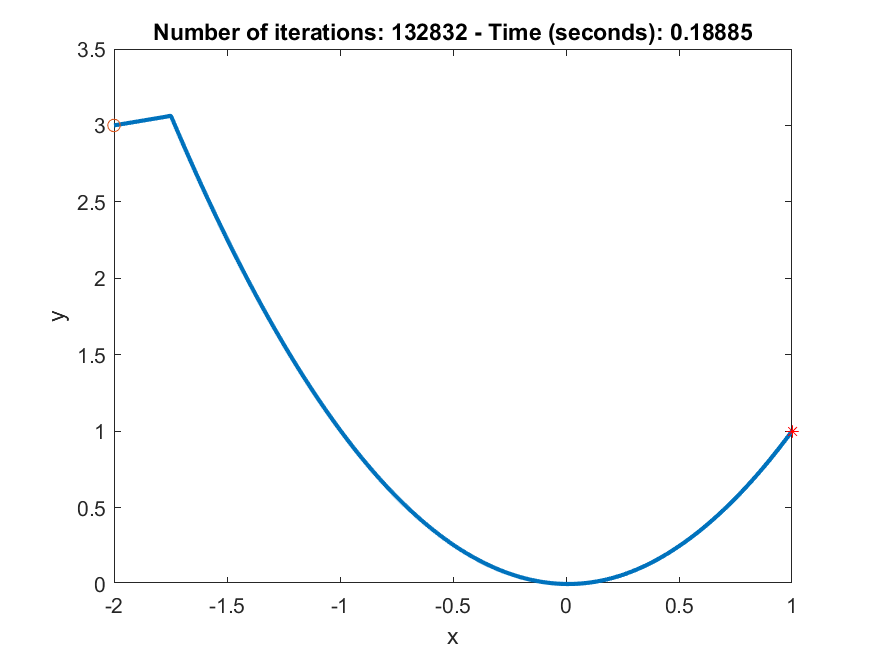
\includegraphics[scale=0.5]{econ714_homework1_question3_plot_cong_3.png}}
       \subfloat{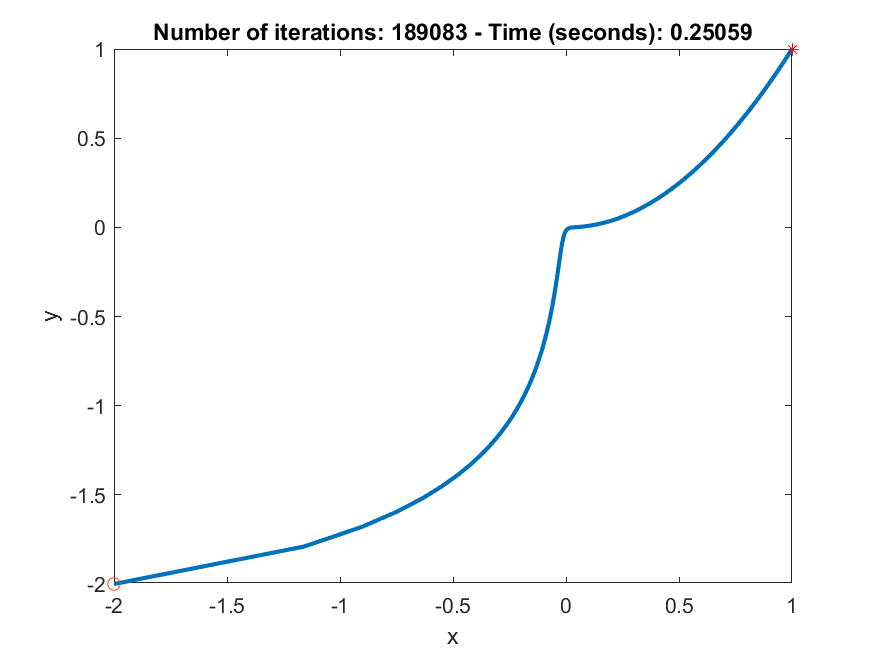
\includegraphics[scale=0.5]{econ714_homework1_question3_plot_cong_4.png}}
        \caption{Conjugate Descent Method} 
        \label{conj_descent}
    \end{figure}
        
    \end{itemize}
    
    
    
    
    % Exercise 4  
    
    \medskip
    \medskip
    \section*{Question 4}   
    \medskip
    
    The code \textit{econ714\_homework1\_question4\_question5.m} generates the output of this problem. This code uses functions \textit{sp\_objective\_function.m} and \textit{spp\_solution.m}. The first function returns the objective function of the social planner and the second function implements the algorithm that solves the social planner problem. Before showing the results, we describe what the algorithm does. 
    
    \begin{itemize}
        \item Let the social planner know the vector of parameters $\alpha$ a vector of weights $\lambda$ and a matrix of preference parameters called $\omega$. Additionally, she knows the total endowment of each good. 
        
        \item She takes the total endowment of each good and divides it between the number of agents of the economy. If the problem was symmetric (including the weights the social planner gives to each agent) we know that the solution would be to divide the total endowment of each good evenly. We are interested in the cases where the problem is not fully symmetric. Divide the total endowment of each good by the number of people in the economy. This is the initial guess of the algorithm. 
        
        \item Start with good $1$. Choose two people at random: we will reallocate a random amount of good $1$ between them. Call $x_{\text{star}}$ the bundle after reallocation. For this we need to tell the social planer the standard deviation of the random variable we are using to make the reallocation. Check that the consumption is not negative and make sure that we are dividing the total endowment of the good (the social planner does not want to waste a single unit). 
        
        \item Once we determine the random amount we want to reallocate, define the next bundle as a Bernoulli random trial between the previous bundle and the one with the reallocation. Let $p = \min\{1,f(x_{\text{star}}) / f(x_{\text{prev}})\}$ be the parameter of the Bernoulli random trail where getting $x_{\text{star}}$ is a success. 
        
        \item If there was an improvement in the objective function, keep the draw. If there was no improvement, disregard it.  
        
        \item Repeat this process for goods $j = 2,\dots,m$. 
        
        \item If we see $100000$ iterations without improvements, stop. This number could be modified to address the fact that having more goods automatically increases the number of iterations. 
    \end{itemize}
    
    Although the algorithm is slow because it performs a lot of iterations, it can handle asymmetries and a higher number of agents and goods. Consider a total endowment of $100$ for each good, let's see how the social planner reallocates it under different parameter values for the case $m=n=3$. 
    
    \begin{itemize}
        \item Let $\omega_j^i = \omega = -2$ for every agent and good. Include heterogeneity in the weights and the parameter $\alpha_j$. In particular, $\lambda = (1,2,3)$ and $\alpha = (3,2,1)$. Table (\ref{table_ex4_cons2}) shows the efficient allocation. These results make sense because the problem is fairly symmetric and the social planner values the utility of individual $3$ the most. The last column of the table has the equilibrium prices. Note that the value of $\alpha$ only matters for the equilibrium prices, but it does not matter for the efficient allocation. The reason behind this is that $\alpha_j$ is the same for every individual. So if we repeat this exercise with $\alpha = (1,1,1)$ we get the same allocation and an equilibrium price vector of $p^* = (1,1,1)$. 
        
        \begin{table}[!htbp]
            \centering
            \caption[Short Caption for LoT]{Allocations for $\omega_i^j=-2$, $\alpha=(3,2,1)$ and $\lambda=(1,2,3)$}\label{table_ex4_cons2}
            \csvautotabular{econ714_homework1_question4_output_cons_2.csv}
        \end{table}
        
        \item Now let $\omega_j^i<0$ be random, $\alpha = (1,1,1)$ and $\lambda = (1,2,3)$. Table (\ref{table_ex4_cons4}) shows the results: the left panel includes the values of $\omega_j^i$ and the right panel the allocation. We see that the higher the value of $\omega_j^i$ (the closer it is to zero) the more consumption agent $i$ gets of good $j$. This makes sense because higher values of $\omega_j^i$ are associated with higher marginal utility to the right of the point $x=1$. Also remember that this social planer likes person $i=3$ the most so she is willing to give person $i=3$ more units. 
        
        \begin{table}[!htbp]
            \centering
            \small
            \caption[Short Caption for LoT]{Allocations for random $\omega_i^j$, $\alpha=(1,1,1)$ and $\lambda=(1,2,3)$}\label{table_ex4_cons4}
             
            
            \csvautotabular{econ714_homework1_question4_output_omega_4.csv}
             \csvautotabular{econ714_homework1_question4_output_cons_4.csv}
        \end{table}
        
        
    \end{itemize}
    
    Now let's jump to the case $m=n=10$. Again there are $100$ units of each good to allocate. 
    
    \begin{itemize}
        \item Let $\omega_j^i = \omega = -2$ for everyone and every good. Here $\alpha$ is a vector of ones and $\lambda = (1,2,3,4,5,6,7,8,9,10)$. So the social planner values agent $i=10$ utility the most. In table (\ref{table_ex4_cons5}) we see that the algorithm can handle this case but we lose precision. Maybe we should increase the number of iteration before stopping, provided that we have more iterations because there are more goods now. Every individual consume the same of each good because the problem is symmetric except for the weights of the social planner. Note that in the competitive equilibrium we get that all the relative prices are the same. This makes sense because the problem is symmetric, the social planner is the one who introduces the asymmetry having different weights. 
        
        
        \begin{table}[!htbp]
            \centering
            \tiny 
            \caption[Short Caption for LoT]{Allocations for $\omega_i^j=-2$, $\alpha$ symmetric and $\lambda=(1,2,3,4,5,6,7,8,9,10)$}\label{table_ex4_cons5}
            \csvautotabular{econ714_homework1_question4_output_cons_5.csv}
        \end{table}
        
        \item Finally let $\omega_j^i<0$ be random, $\alpha$ be a vector of ones and again let the weights differ $\lambda =(1,2,3,4,5,6,7,8,9,10)$. Table (\ref{table_ex4_cons6}) shows the results: the first table has the values of $\omega_i^j$ and the second table has the solution of the social planner problem. For a given agent, the social planner allocates more units if the $\omega_j$ is higher (closer to zero). And again we see a preference towards individuals to the right because we are giving them more weight. 
        
        \begin{table}[!htbp]
            \centering
            \tiny 
            \caption[Short Caption for LoT]{Allocations for random $\omega_j^i$, $\alpha$ symmetric and $\lambda=(1,2,3,4,5,6,7,8,9,10)$}\label{table_ex4_cons6}
            \csvautotabular{econ714_homework1_question4_output_omega_6.csv}
            
            \vspace*{0.5 cm}
            \csvautotabular{econ714_homework1_question4_output_cons_6.csv}
        \end{table}
    \end{itemize}
    
    
    
    % Exercise 5  
    
    \medskip
    \medskip
    \section*{Question 5}   
    \medskip
    
    The equilibrium prices are computed using the function \textit{eq\_prices.m}. The same file \textit{econ714\_homework1\_question4\_question5.m} generates the output. Tables (\ref{table_ex4_cons2}), (\ref{table_ex4_cons4}), (\ref{table_ex4_cons5}) and (\ref{table_ex4_cons6}) show the equilibrium prices for the cases we presented in question $4$, but here we include some additional cases that are interesting. Before, the initial endowment was the same for all goods and also sometimes the value of $\alpha$ was unchanged. Here it will be interesting to vary the initial endowment to make some good more or less scarce and see how that affects the equilibrium prices. We describe what the algorithm does to compute the equilibrium prices. We use the Newton-Raphson method for nonlinear systems of equations. 
    
    \begin{itemize}
        \item Guess a price vector. Start with one person and calculate her income using the guess. The initial guess for $x^i=(x^i_1,\dots, x^i_m)$ is the income divided by $m\cdot p_j$. This would be the solution if the utility function was Cobb Douglas. 
        \item Now calculate the first order condition at this value of $x^i$. This a vector valued function $F(\cdot)$ (with $m$ dimensions) where the first equation is the budget constraint and we have eliminated the Lagrange multiplier. Calculate the norm of $F(\cdot)$: as long as the norm is higher than our tolerance level, we continue iterating. 
        \item Calculate the Jacobian matrix $J$ of the system and define a possible step as $-J^{-1}\cdot F(\cdot)$. Change the step if it is too high: we don't want to move too fast. See equation (\ref{systemF}) for more details about the system. 
        
        \item Update the point $x^i$ and start again. After iterating we get the individual demand of person $i$. 
        
        \item Repeat for everyone and get the aggregate demand. 
        
        \item If the aggregate demand of a good is greater than the aggregate endowment, randomly increase the price of that good. Similarly, if the aggregate demand of a good is smaller than its aggregate endowment, randomly decrease the price. Here we use the absolute value of a zero mean normal random variable. We let the standard deviation depend on the excess demand so that the price changes makes sense in every iteration (they get smaller as we approach the solution). Also we do not want the standard deviation to be too large because it may cause troubles with the matrix $J$, so we set the maximum standard deviation equal to $1$. 
        
        \item Start the process again and repeat until the aggregate demand and aggregate endowment are close to each other. 
    \end{itemize}
    
    The algorithm is slow, but it seems to work at least when the heterogeneity is not too high. When the values of $\omega_i^j$ are very different from each other, the algorithm has troubles inverting the Jacobian. We tried to address this by forcing the method to take smaller steps so that the matrix does not change too much from iteration to iteration. In particular, the maximum step in a given direction cannot exceed $5\%$ of the maximum amount the agent could buy of that good, that is, $0.05 \cdot m/p_j$, where $m$ is the income. Similarly, we made sure that the draws for the new price vector do not have a large standard deviation. Table (\ref{table_ex5}) presents the equilibrium prices of seven possible scenarios. In all of them there are $3$ people and $3$ goods.
    
    
    \begin{enumerate}
        \item First $\alpha = (3,2,1)$, there are $100$ units of each good. Person $i$ owns all the endowment of good $j=i$. Here we see that good $1$ is relatively more expensive because it is more desirable. We use $\omega_j^i=-2$ for all $i$ and $j$. 
        \item Redistributing the initial endowment from the first scenario does not change the equilibrium price vector. Here everything is the same as before but now the initial endowment is $100/3$ for each good and each person. 
        \item Now there are $90$ units of good $1$, $100$ units of good $2$ and $120$ units of good $3$ owned by agents $1$, $2$ and $3$ respectively. 
        \item Same as the previous one but the initial endowment is shared equally between everyone. we see that the equilibrium prices do not change.  
        \item Now we go back to scenario $1$ but we vary $\omega$. Person $i$ has the same $\omega_j^1 = -2$ for every good, person $2$ has $\omega_j^2 = -2.05$ for every good and person $3$ has $\omega_j^3 = -2.1$ for every good. We see that the equilibrium prices do not change when comparing to the first scenario. This makes sense because the preferences are homothetic. 
        \item Now good $1$ has $\omega_1^i=-2$ for every individual, good $2$ has $\omega_2^i=-2.05$ for everyone and good $3$ has $\omega_3^i=-2.1$ for everyone. Now we see differences in the equilibrium prices. 
        
        \item Same as scenario $1$ but now we use $\alpha = (1,2,3)$. Note that $p^* = \alpha$. 
    \end{enumerate}
    
    
        \begin{table}[!htbp]
            \centering
            \caption[Short Caption for LoT]{Equilibrium prices of $6$ possible scenarios}\label{table_ex5}
            \csvautotabular{econ714_homework1_question5_output.csv}
        \end{table}
        
        
    For each individual $i=1,\dots, n$ we solve the following system. We omit the superscripts that refer to the agent. $F(x)$ is $m\times 1$. We eliminate the Lagrange multiplier by using the first order condition of the agent. 

    \begin{align}\label{systemF}
    \begin{cases}
        F_1(x) & = p_1x_1 + \dots + p_mx_m - p_1e_1 -\dots - p_me_m = 0 \\  F_j(x) & = \frac{\alpha_j}{\alpha_1} \cdot \frac{x_j^{\omega_j}}{x_1^{\omega_1}} - \frac{p_j}{p_1} = 0 \quad\text{for}\quad j = 2,\dots,m
    \end{cases}
    \end{align}
    
    The Jacobian of the system looks like this. we express it in terms of $F(x)$ to help with the computation. 
    
    \begin{align*}
        J & = \begin{pmatrix} p_1 & p_2 & \dots & p_m \\ -\frac{\omega_1}{x_1}  F_2(x) & \frac{\omega_2}{x_2} F_2(x) & \dots & 0 \\ \dots & \dots & \dots &\dots \\ -\frac{\omega_1}{x_1} F_m(x) & 0 & \dots & \frac{\omega_m}{x_m} F_m(x) \end{pmatrix}
    \end{align*}
    
    
    
  

    

%\hfill

%\pagebreak 

%\pagestyle{empty}

%\section*{Codes}


    %\begin{lstlisting}[language= R]
    
%-


    
    %\end{lstlisting}

    
    
 \end{document}
 